\documentclass[slides.tex]{subfiles}
\begin{document}
\section{Example}
\begin{frame}{Base-game: Game of Chicken}
\centering
\renewcommand{\arraystretch}{1.2}
\begin{tabular}{c|cc}
           & \textbf{Straight} & \textbf{Move} \\ \hline
\textbf{Straight} & $-1,\,-1$ & $\;\;1,\,-\tfrac12$ \\[2pt]
\textbf{Move}   & $-\tfrac12,\,1$ & $\;\;0,\,0$
\end{tabular}
\medskip

\begin{itemize}
  \item Two pure Nash equilibria (off-diagonal).  
  \item Unique symmetric equilibrium: Straight w.p.\ $2/3$.
\end{itemize}
\end{frame}
\begin{frame}{Game with Commitment}
\vspace{1ex}
\begin{itemize}
    \item Initial period before the base game
    \vspace{1ex}
    \item Each player simultaneously chooses one of:
    \vspace{0.5ex}
        \begin{itemize}
          \item \textbf{Commit} to any normal-form strategy of the base game
          \vspace{0.5ex}
          \item \textbf{Wait} to observe the opponent’s commitment before choosing
        \end{itemize}
\end{itemize}
\end{frame}

\begin{frame}{Game tree}
    \begin{figure}[ht]
    \centering
    \resizebox{0.8\textwidth}{!}{%
        \begin{tikzpicture}
        %--- Macros with Updated Labels ---
        \newcommand{\firststage}[2]{%
            % Nodes for Player 2 at period 1 (following Player 1's move)
            \node (#11) [circle, draw, below of=#1, xshift=-#2, yshift=\yshift]{};
            \node (#12) [circle, draw, below of=#1, xshift=0, yshift=\yshift]{};
            \node (#13) [circle, draw, below of=#1, xshift=#2, yshift=\yshift]{};
            % Branches: left branch is Wait (W); the others are S and M.
            \draw (#1) -- (#11) node[midway, left] {W};
            \draw (#1) -- (#12) node[midway, left] {S};
            \draw (#1) -- (#13) node[midway, right] {M};
        }
        
        \newcommand{\aftercommit}[2]{%
            % Node following a committed action (only one possible continuation)
            \node (#11) [circle, draw, below of=#1, xshift=0, yshift=\yshift]{};
            \draw (#1) -- (#11) node[midway, right] {#2};
        }
        
        \newcommand{\afternocommit}[4]{%
            % Node for the noncommitted branch (with two possible moves)
            \node (#11) [circle, draw, below of=#1, xshift=-#2, yshift=\yshift]{};
            \node (#12) [circle, draw, below of=#1, xshift=#2, yshift=\yshift]{};
            \draw (#1) -- (#11) node[midway, left] {#3};
            \draw (#1) -- (#12) node[midway, right] {#4};
        }
        
        %--- Define Shift Variables ---
        \newcommand{\xshiftA}{5cm}           % For first stage    
        \newcommand{\xshiftfollowone}{0.25cm}  % For third stage (single branch)
        \newcommand{\xshiftC}{0.5cm}          % For fourth stage
        \newcommand{\xshiftlabel}{-10cm}      % For labels
        \newcommand{\yshift}{-0.5cm}
        
        %--- Root Node (Player 1) ---
        \node (root) at (0,0) [circle, draw] {};
        
        % Player 1’s initial decision: Wait, commit to S, or commit to M
        \node (child1) [circle, draw, below of=root, xshift=-\xshiftA-1cm, yshift=\yshift]{};
        \node (child2) [circle, draw, below of=root, xshift=0cm, yshift=\yshift]{};
        \node (child3) [circle, draw, below of=root, xshift=\xshiftA-1cm, yshift=\yshift]{};
        
        \draw (root) -- (child1) node[midway, above left] {Wait (W)};
        \draw (root) -- (child2) node[midway, left] {S};
        \draw (root) -- (child3) node[midway, right] {M};
        
        %--- Player 2’s First Stage Decisions ---
        \firststage{child1}{2cm}
        \firststage{child2}{1cm}
        \firststage{child3}{1cm}
        
        %--- t = 2, Player 1's Decisions after Not Committing ---
        \afternocommit{child11}{0.8cm}{S}{M}
        \afternocommit{child12}{\xshiftfollowone}{S}{M}
        \afternocommit{child13}{\xshiftfollowone}{S}{M}
        
        %--- t = 2, Player 1's Decisions after Having Committed ---
        \aftercommit{child21}{S}
        \aftercommit{child22}{S}
        \aftercommit{child23}{S}
        \aftercommit{child31}{M}
        \aftercommit{child32}{M}
        \aftercommit{child33}{M}
        
        %--- t = 2, Player 2's Subsequent Decisions ---
        \afternocommit{child111}{\xshiftC}{S}{M}
        \afternocommit{child112}{\xshiftC}{S}{M}
        \aftercommit{child121}{S}
        \aftercommit{child122}{S}
        \aftercommit{child131}{M}
        \aftercommit{child132}{M}
        
        \afternocommit{child211}{0.5cm}{S}{M}
        \aftercommit{child221}{S}
        \aftercommit{child231}{M}
        
        \afternocommit{child311}{0.5cm}{S}{M}
        \aftercommit{child321}{S}
        \aftercommit{child331}{M}
        
        %--- Define Information Sets and Labels ---
        \begin{pgfonlayer}{background}
            \node [draw=black, dashed, fit=(child1)(child3), inner sep=2pt] {};
            \node [draw=black, dashed, fit=(child111)(child112), inner sep=2pt] {};
            \node [draw=black, dashed, fit=(child121)(child122), inner sep=2pt] {};
            \node [draw=black, dashed, fit=(child131)(child132), inner sep=2pt] {};
            
            \node (P1label1) [draw=none, left of=root, xshift=\xshiftlabel] {Player 1};
            \node (P2label1) [draw=none, below of=P1label1, yshift=\yshift] {Player 2};
            \node (P1label2) [draw=none, below of=P2label1, yshift=\yshift] {Player 1};
            \node (P2label2) [draw=none, below of=P1label2, yshift=\yshift] {Player 2};
        \end{pgfonlayer}
    \end{tikzpicture}
    }
    \caption{The Game Tree for the 2×2 Game of Chicken}
    \label{fig:game tree}
\end{figure}
\end{frame}
\begin{frame}{Commitment can be bad}
Symmetric equilibrium of the game:
\vspace{0.8em}

  \begin{columns}[T,onlytextwidth]
    %------------- Left column -----------------
    \column{0.48\textwidth}
    \textbf{Without commitment}
    \begin{itemize}
      \item Choose Straight with probability $\tfrac{2}{3}$
      \item Expected payoff of $-\tfrac{1}{3}$
    \end{itemize}

    %------------- Right column ----------------
    \column{0.48\textwidth}
    \textbf{With commitment}
    \begin{itemize}
      \item Commit Straight with probability $\tfrac{8}{11}$
      \item Expected payoff of $-\tfrac{5}{11}$
    \end{itemize}
  \end{columns}
\end{frame}

\begin{frame}{Intuition}
  \centering
  {\large Commitment transforms the game into one with worse payoffs!}

  \vspace{3em}  % adjust this to add more or less vertical space

  % Shrink both tables plus arrow to fill the text width
  \resizebox{\textwidth}{!}{%
    \renewcommand{\arraystretch}{1.25}%
    \begin{tabular}{ccc}
      % first table
      \begin{tabular}{c|cc}
             & \textbf{S} & \textbf{M} \\ \hline
        \textbf{S} & $-1,\,-1$ & $\;1,\,-\tfrac12$ \\[2pt]
        \textbf{M}     & $-\tfrac12,\,1$ & $\;0,\,0$
      \end{tabular}
      &
      % arrow
      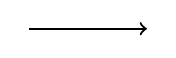
\begin{tikzpicture}[baseline=(current bounding box.center)]
        \draw[thick,->] (0,0) -- (1.5,0);
      \end{tikzpicture}
      &
      % second table
      \begin{tabular}{c|cc}
             & \textbf{Commit S} & \textbf{Wait} \\ \hline
        \textbf{Commit S} & $-1,\,-1$ & $\;1,\,-\tfrac12$ \\[2pt]
        \textbf{Wait}     & $-\tfrac12,\,1$ & $\;-\tfrac{1}{3},\,-\tfrac{1}{3}$
      \end{tabular}
    \end{tabular}%
  }
\end{frame}
\end{document}